\documentclass{article}
\usepackage[utf8]{inputenc}
\usepackage{amsmath}
\usepackage{amsfonts}
\usepackage{amssymb}
\usepackage{graphicx}
\usepackage{listings}
\usepackage{xcolor}
\usepackage{minted}
\usepackage{biblatex}
\addbibresource{references.bib}

\title{Dynamic Linear Gaussian State-Space Models}
\author{[Your Name]}
\date{}

\begin{document}
\maketitle

\section{Motivating Example and Definition of Dynamic Linear Gaussian State-Space Models}
Dynamic Linear Gaussian State-Space Models (DLGSSMs) are a cornerstone of modern time series analysis, allowing for the modeling of systems where we can only observe indirect, noisy measurements over time. They are widely applicable in various fields such as economics, engineering, and ecology.

\subsection{Motivating Example: Object Tracking}
Consider tracking the position and velocity of an object over time using a GPS device. The measurements are subject to noise and may not be directly observed. This is a classic example where DLGSSMs excel.

\subsection{Notation and Definition}
Let $\left(X_0, \ldots, X_T\right)$ be a sequence of continuous random variables taking values in $\mathbb{R}^{d_x}$, corresponding to the hidden state of interest, and $\left(Y_1, \ldots, Y_T\right)$ be a sequence of continuous random variables taking values in $\mathbb{R}^{d_y}$ (observations). The linear Gaussian state-space model is defined as, for $t=1, \ldots, T$
$$
\begin{aligned}
X_t & =F_t X_{t-1}+G_t V_t \\
Y_t & =H_t X_t+W_t
\end{aligned}
$$

where the random variables $\left(X_0, V_1, V_2, \ldots, V_T, W_1, W_2, \ldots, W_T\right)$ are independent with $X_0 \sim \mathcal{N}\left(\mu_0, \Sigma_0\right)$ and for $t=1, \ldots, T$,
$$
\begin{aligned}
V_t & \sim \mathcal{N}\left(0, Q_t\right) \\
W_t & \sim \mathcal{N}\left(0, R_t\right)
\end{aligned}
$$
with
\begin{itemize}
    \item $X_t$ is the hidden state at time $t$
    \item $Y_t$ is the observation at time $t$
    \item $V_t$ is the state noise at time $t$
    \item $W_t$ is the observation noise at time $t$
    \item $F_t$ is the $d_x \times d_x$ state transition matrix
    \item $G_t$ is the $d_x \times d_v$ noise transfer matrix
    \item $H_t$ is the $d_y \times d_x$ observation matrix
\end{itemize}

Under the above assumptions, the sequence $\left(X_0, X_1, Y_1, \ldots, X_T, Y_T\right.$ ) is a (continuous-state) hidden Markov model, which can be represented graphically as in Figure 2. If $G_t Q_t G_t^{\top}$ has full rank, the joint pdf $p\left(x_{0: T}, y_{1: T}\right)$ factorizes as
$$
p\left(x_{0: T}, y_{1: T}\right)=p\left(x_0\right) \prod_{t=1}^T p\left(y_t \mid x_t\right) p\left(x_t \mid x_{t-1}\right)
$$
where
$$
\begin{aligned}
p\left(x_t \mid x_{t-1}\right) & =\mathcal{N}\left(x_t ; F_t x_{t-1}, G_t Q_t G_t^{\top}\right) \\
p\left(y_t \mid x_t\right) & =\mathcal{N}\left(y_t ; H_t x_t, R_t\right)
\end{aligned}
$$

\section{Inference in Dynamic Linear Gaussian SSMs}
Inference in DLGSSMs typically involves learning about the hidden states given the observations, which can be achieved through the Kalman filter and smoother.

\subsection{The Kalman Filter}

The Kalman filter is a recursive algorithm used for estimating the state of a linear dynamic system from a series of noisy measurements. It is named after Rudolf E. Kálmán, one of the primary developers of its theory.

\subsubsection{Definitions and Notation}

The Kalman filter operates on the Gaussian state-space model and involves two sets of equations: the state equation and the observation equation. The state at time \( t \) is denoted by \( X_t \), and the observations up to and including time \( t \) are denoted by \( Y_{1:t} \). The key quantities computed by the Kalman filter are:

- \( \mu_{t|t-1} \): the predicted mean state estimate at time \( t \) given observations up to time \( t-1 \),
- \( \Sigma_{t|t-1} \): the predicted covariance estimate of the state estimate uncertainty at time \( t \) given observations up to time \( t-1 \),
- \( \mu_{t|t} \): the updated mean state estimate at time \( t \) after observing \( Y_t \),
- \( \Sigma_{t|t} \): the updated covariance estimate of the state estimate uncertainty at time \( t \) after observing \( Y_t \).

The filter proceeds by alternating between a prediction step and an update step to incorporate the new observation.

\subsubsection{Intuitive Explanation of the Kalman Filter}

At its core, the Kalman filter maintains a belief about the state of the system as a probability distribution. Each time step involves two phases:
- \textbf{Prediction}: Before a new measurement is taken, the Kalman filter uses a model of the system to predict what the next state will be, as well as the uncertainty of that prediction.
- \textbf{Update}: Once a new measurement is available, it updates its estimate of the state by combining the prediction with the new measurement.

The magic of the Kalman filter lies in its ability to optimally balance the uncertainty in the model's predictions with the noise in the measurements, using a factor called the Kalman gain.

\subsubsection{Usefulness and Pros and Cons}

The Kalman filter is incredibly useful in situations where data is noisy and uncertain. It excels in providing real-time updates to estimates, which is critical in navigation systems like GPS and automated vehicles. Moreover, it's efficient in terms of computational resources, which allows it to run on hardware with limited processing power.

However, the Kalman filter has some limitations. It assumes that the system is linear and that the noise is Gaussian, which may not hold true for all systems. Additionally, it does not handle the case where the model of the system changes over time or is not well known.

\subsubsection{Step by Step Example of Kalman Filtering}

Let's consider a step by step example based on the second screenshot provided:

1. \textbf{Prediction Step}
   - Calculate the predicted state estimate: \( \mu_{t|t-1} = F_{t-1}\mu_{t-1|t-1} \)
   - Calculate the predicted estimate covariance: \( \Sigma_{t|t-1} = F_{t-1}\Sigma_{t-1|t-1}F_{t-1}^T + G_{t-1}Q_{t-1}G_{t-1}^T \)

2. \textbf{Update/Correction Step}
   - Calculate the Kalman gain: \( K_t = \Sigma_{t|t-1}H_t^T(S_t)^{-1} \)
   - Update the estimate with the measurement: \( \mu_{t|t} = \mu_{t|t-1} + K_t\nu_t \)
   - Update the estimate covariance: \( \Sigma_{t|t} = (I - K_tH_t)\Sigma_{t|t-1} \)

In this process, \( \nu_t \) is the residual or innovation, which is the difference between the actual observation and the predicted observation. \( S_t \) is a term that comes from the innovation covariance, representing the uncertainty of the observation. This step-by-step process is repeated at each time step, refining the 
\begin{figure}
    \centering
    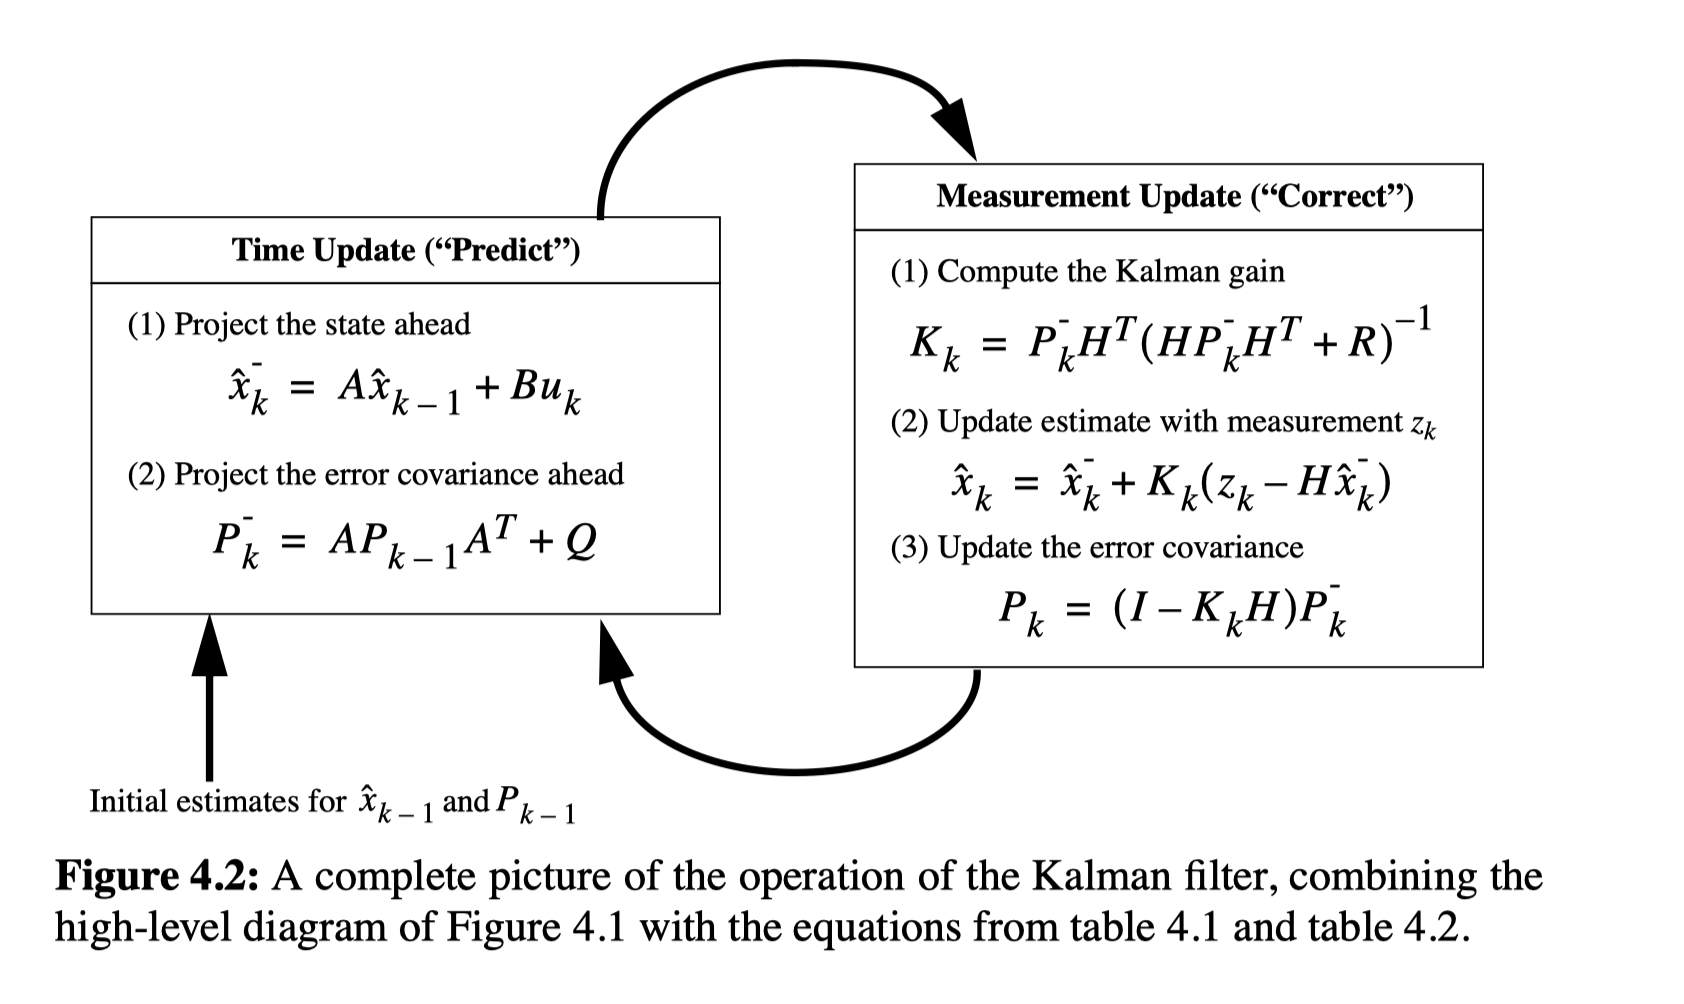
\includegraphics[width=1\linewidth]{overviews/HMM/figures/Filter visuals.png}
    \caption{Figure from \cite{welch_introduction_nodate} }
    \label{fig:enter-label}
\end{figure}

\subsection{The Kalman Smoother}

The Kalman smoother, an extension of the Kalman filter, is a  algorithm used to estimate the states of a process retrospectively. While the Kalman filter operates recursively to estimate the current state based on past observations, the smoother takes advantage of both past and future observations to refine these estimates. This process yields a more accurate reconstruction of the state trajectory over time.

\subsubsection{Definitions and Notation}
The smoother operates within the state-space model framework and utilizes the following definitions and notation (as per the screenshot provided):

- \(\mu_{t|T}\) represents the smoothed estimate of the state at time \(t\) given all observations up to time \(T\).
- \(\Sigma_{t|T}\) denotes the smoothed error covariance matrix.
- The smoothing pdf at time \(t\) is given by \(p(x_t|y_{1:T}) = \mathcal{N}(\mu_{t|T}, \Sigma_{t|T})\).
- The smoothed estimates are calculated using the forward recursion of the Kalman filter, followed by a backward recursion to incorporate future observations.

\subsubsection{Intuitive Explanation}
The Kalman smoother can be thought of as a hindsight tool that revises state estimates after considering the entire dataset. Imagine watching a movie: the Kalman filter gives you an impression of the plot as the story unfolds, while the smoother lets you reinterpret earlier scenes after you’ve seen the whole film.

\subsubsection{Utility and Considerations}
The Kalman smoother is incredibly useful when the entire dataset is available, as it can provide the best linear unbiased estimates (BLUE) of the states. It's particularly beneficial in scenarios where delayed but accurate state estimation is preferable to real-time but less accurate filtering.

However, it's important to note that the smoother's reliance on the entire dataset makes it unsuitable for real-time applications. It also requires more computational resources than the filter alone, due to the necessity of a backward pass through the data.

\subsubsection{Step-by-Step Example}
Consider a simple scalar example of a random walk observed with noise, similar to the one presented in the screenshot:

- State equation: \(X_t = X_{t-1} + v_t\)
- Observation equation: \(Y_t = X_t + w_t\)
- Initial conditions: \(X_0 \sim \mathcal{N}(0,1)\), \(v_t \sim \mathcal{N}(0,Q)\), \(w_t \sim \mathcal{N}(0,R)\)

For the smoother, we first run the Kalman filter through all time points to get the filtered estimates \(\mu_{t|t}\) and \(\Sigma_{t|t}\). Then, we apply the backward recursion:

- Smoothing step: \( \mu_{t|T} = \mu_{t|t} + J_t(\mu_{t+1|T} - \mu_{t+1|t}) \)
- Covariance smoothing: \( \Sigma_{t|T} = \Sigma_{t|t} + J_t(\Sigma_{t+1|T} - \Sigma_{t+1|t})J_t^T \)

Where \( J_t \) is the smoother gain, calculated as:
\( J_t = \Sigma_{t|t}F_{t}^T\Sigma_{t+1|t}^{-1} \).

Applying this process to the given example would involve first using the Kalman filter equations to obtain \(\mu_{t|t}\) and \(\Sigma_{t|t}\) for all \(t\), and then working backwards from \(T\) to 1 using the smoother equations to refine these estimates. The result is a set of smoothed estimates that are more accurate than the filtered estimates, as they incorporate information from the entire observation sequence.


\section{Further Literature}
I highly recommend reading the following two intros to the Kalman filter:
\begin{itemize}
    \item \cite{lacey_tutorial_nodate}
    \item \cite{welch_introduction_nodate}
\end{itemize}


\printbibliography
\end{document}